\documentclass{beamer}
\usepackage[ngerman]{babel}
\usepackage[ansinew]{inputenc}
\usepackage{csquotes}
\usepackage{url}
\usepackage{graphicx}
\usepackage{amsmath}
\usepackage{amssymb}
\usepackage{nicefrac}
\usepackage{eurosym}
\usepackage{xcolor}
\usepackage{alltt}
\usepackage{tikz}
\usepackage{ragged2e} 
\usepackage{tabu}
\usetikzlibrary{trees}
\usepackage{calc,color,colortbl,nicefrac}
\newtheorem*{bem}{Bemerkung}
\usepackage{multirow}
\usepackage{tikz}
\usepackage{scalefnt}

%smaller footnotes
\renewcommand{\footnotesize}{\tiny}
%reduce spacing in footnotes
\setlength{\footnotesep}{0em}

%use for inline citation formatting
\newcommand{\textct}[1]{{\textsuperscript{\tiny \color{gray}#1}}}

\newlength{\myX}
\newlength{\myY}

%absolute figure positioning
\usepackage[absolute,overlay]{textpos}
  \setlength{\TPHorizModule}{1mm}
  \setlength{\TPVertModule}{1mm}

%quote environment with reference 
\def\signed #1{{\leavevmode\unskip\nobreak\hfil\penalty50\hskip2em
  \hbox{}\nobreak\hfil(#1)%
  \parfillskip=0pt \finalhyphendemerits=0 \endgraf}}
\newsavebox\mybox
\newenvironment{aquote}[1]
  {\savebox\mybox{#1}\begin{quote}}
  {\signed{\usebox\mybox}\end{quote}}

\definecolor{purp}{HTML}{3333b3}
\definecolor{dgrey}{rgb}{0.8,0.8,0.8}
\definecolor{bgrey}{rgb}{0.95,0.95,0.95}

\usepackage{graphicx}
\graphicspath{{img/}}

\newlength{\stdlength}
% Standardlaenge fuer Skript und Folien
\setlength{\stdlength}{8cm}

\usetheme{Copenhagen}
\usefonttheme{professionalfonts}
\usecolortheme{default}

\bibliography{literature}
\usepackage[style=authoryear, backend=bibtex]{biblatex} 
\addbibresource{literature.bib}

\defbibenvironment{bibliography}
{\list{}
{\setlength{\leftmargin}{\bibhang}%
\setlength{\itemindent}{-\leftmargin}%
\setlength{\itemsep}{6px}%
\setlength{\parsep}{\bibparsep}}}
{\endlist}
{\item \scriptsize}

\definecolor{mygrey}{RGB}{80,80,80}

\setbeamertemplate{headline}
{%
\hfill
\textbf{\insertsection} \
\insertsubsection \
\insertframenumber / \inserttotalframenumber
}
\setbeamertemplate{navigation symbols}{}

\title{Bewegungsvorhersage mittels mobiler Endger�te}
\author{
Sebastian B�r, Frank Rosner
}

\institute{
Martin-Luther-Universit�t Halle-Wittenberg
}
\date{10. Juli 2013}

\begin{document}

\frame{\titlepage 
\parbox{0cm}{\tiny 
\vspace{-30pt}\color{mygrey}
\begin{tabbing}
XXXXXXXXXXXXXXXXXXXXXX\=XXXXXXXXXXX\= \kill \\
\>Veranstaltung:\> "`Seminar zum E-Business"'\\
\\
\>Dozenten:\> Prof. Dr. Ralf Peters\\
\>\> Dr. Thomas W�hner\\
\>\> Sebastian K�hler\\
\>\> Uwe Bretschneider\\

\end{tabbing}
}
}

\begin{frame}
\frametitle{Gliederung}
\tableofcontents
\end{frame}

\section{Einleitung}
\frame{\frametitle{Gliederung} \tableofcontents[currentsection]}

\begin{frame}{Problemstellung}
\begin{itemize}
\item Computer allgegenw�rtig
	\begin{itemize}
	\item[$\Rightarrow$] mobile Endger�te
	\item[$\Rightarrow$] "`ubiquitous computing"'
	\end{itemize}
\item Positionsbestimmung relativ genau m�glich
\end{itemize}

\begin{itemize}
\item wirtschaftlicher Nutzen?
	\begin{itemize}
	\item[$\Rightarrow$] positionsabh�ngige, personalisierte Dienste
	\item[$\Rightarrow$] z.B. Mittagskarte eines Restaurants in der N�he
	\end{itemize}
\end{itemize}

\begin{itemize}
\item Positionsvorhersage statt Positionsbestimmung?
	\begin{itemize}
	\item[$\Rightarrow$] positionsabh�ngige Dienste im Voraus bereitstellen
	\item[$\Rightarrow$] Mittagskarte des Restaurants, wenn ich mich gerade auf dem Weg dorthin befinde
	\end{itemize}
\end{itemize}

\begin{textblock}{70}(100,25)
	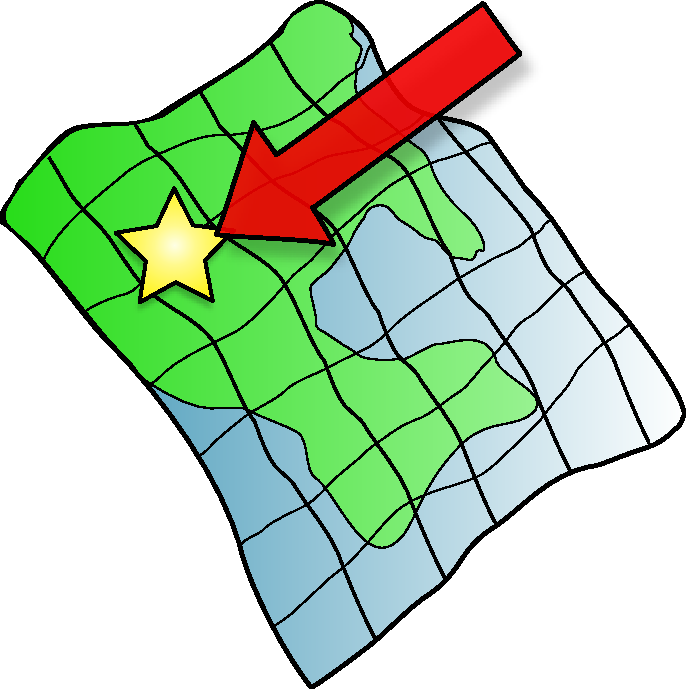
\includegraphics[width=2cm]{ruffled_map.pdf}
\end{textblock}

\end{frame}

\begin{frame}{Zielstellung und Methodik}
\textbf{Zielstellung}
\begin{itemize}
\item Android-App zur Bewegungsdatensammlung entwickeln
\item Auswerten der Positions- und Bewegungsdaten
	\begin{itemize}
	\item[$\Rightarrow$] Visualisierung
	\item[$\Rightarrow$] Vorhersage
	\end{itemize}
\end{itemize}

\vspace*{1em}

\textbf{Methodik}
\begin{itemize}
\item Softwareentwicklung
\item Datensammlung
\item Statistische Auswertung
\end{itemize}
\end{frame}

\section{Datensammlung}
\frame{\frametitle{Gliederung} \tableofcontents[currentsection]}
\begin{frame}{Android �berblick}
\begin{figure}[h]
\centering
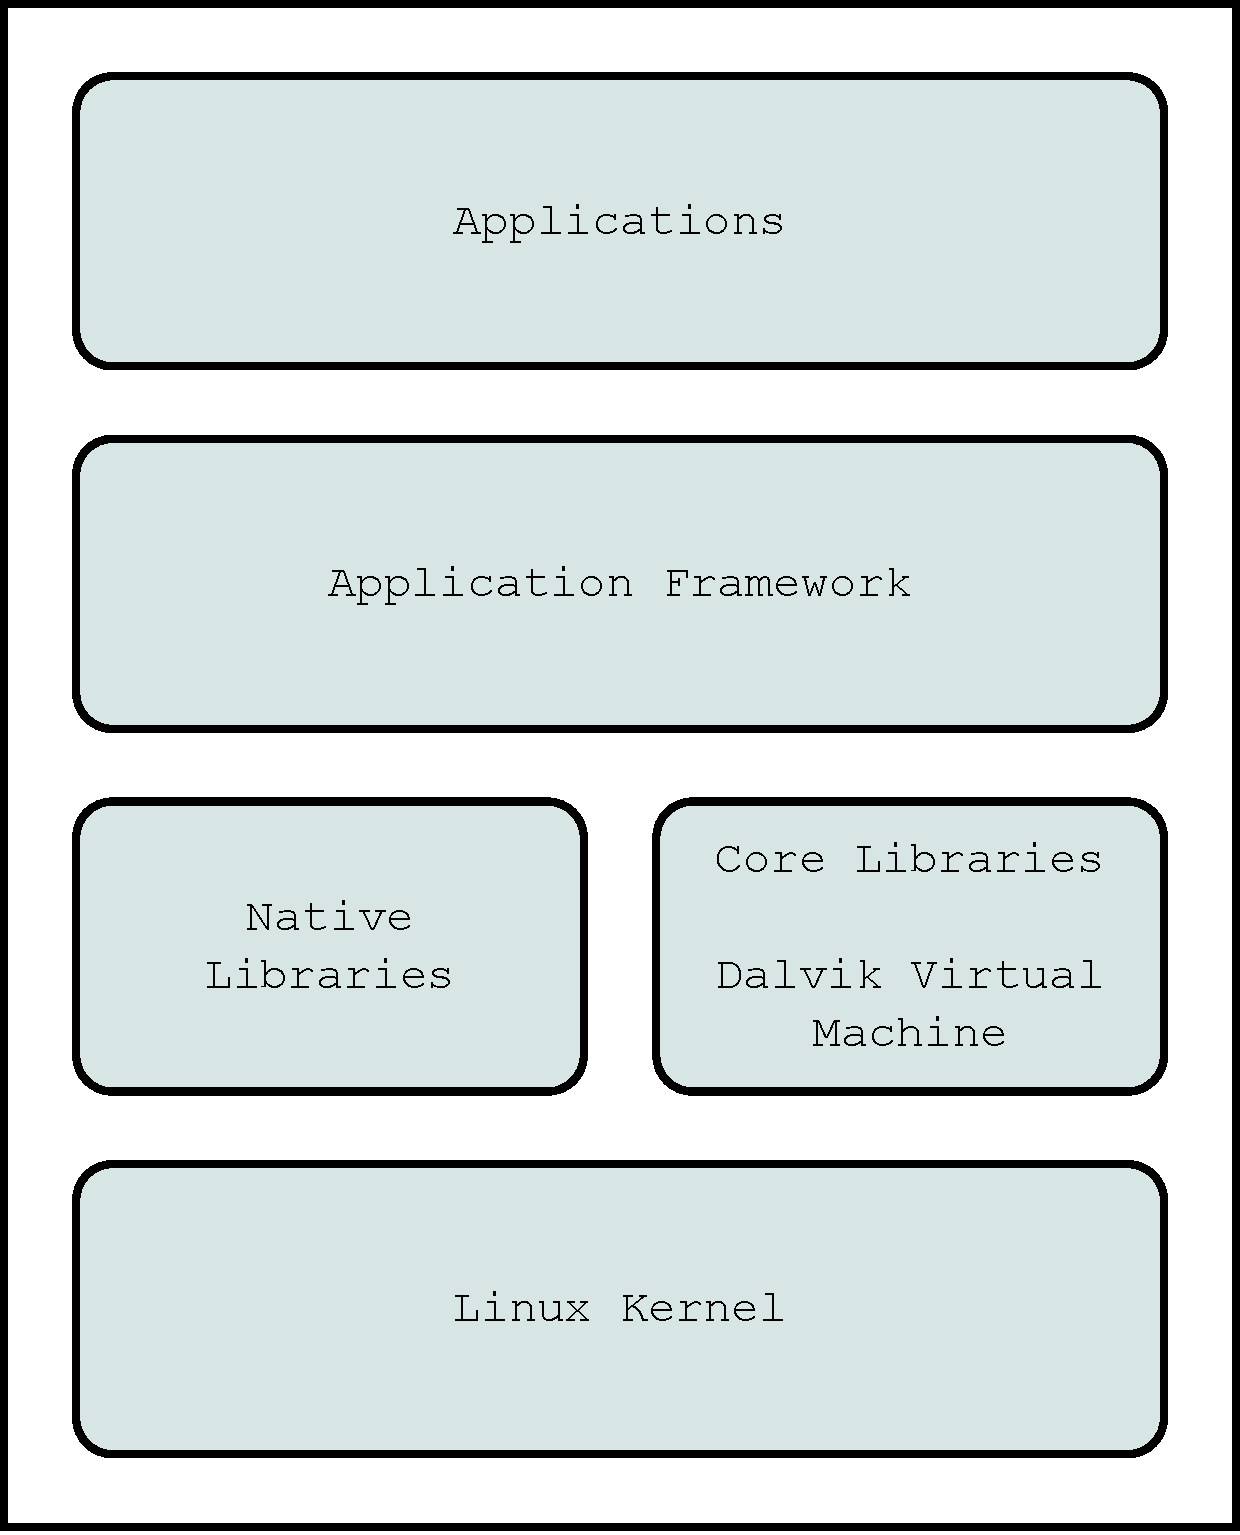
\includegraphics[height=60mm]{android_stack.pdf}
\newline
\medskip
\hfill \tiny \cite[Vgl.][S. 8]{gargenta2011learning} \hspace*{23em}
\end{figure}
\end{frame}

\begin{frame}{Android-SDK}
\begin{itemize}
\item enth�lt Eclipse als IDE
\item Debug-Treiber zur Anbindung von Ger�ten
\item Emulator zum Testen
\item Debug-Monitor
\item Layout-Editor
\item SQLite Datenbank-Treiber
\item XML-Editor
\newline
\medskip
\hfill \tiny \cite[Vgl.][]{google2013tools} \hspace*{4em}
\end{itemize}
\end{frame}

\begin{frame}{Aufbau einer Applikation}
\begin{itemize}
\item \textbf{Activities} �bernehmen Darstellung des User-Interface sowie Ausf�hrung von Logik
\item \textbf{Services} verarbeiten Aufgaben im Hintergrund
\item \textbf{Intents} sind abstrakte Beschreibungen von Operationen, die eine App ben�tigt und eine andere anbieten kann
\item \textbf{BroadcastReceiver} warten auf Intents und verarbeitet diese
\item \textbf{AndroidManifest} enth�lt Informationen dar�ber welche Android-Versionen unters�tzt werden, Versionen der App, welche Berechtigungen n�tig sind
\item dar�ber hinaus wird ein \textbf{Layout}-XML ben�tigt
\newline
\medskip
\hfill \tiny \cite[Vgl.][]{google2013fundamentals} \hspace*{4em}
\end{itemize}
\end{frame}

\begin{frame}{Aufbau AndroidDataCollection}
\begin{figure}[h]
\centering
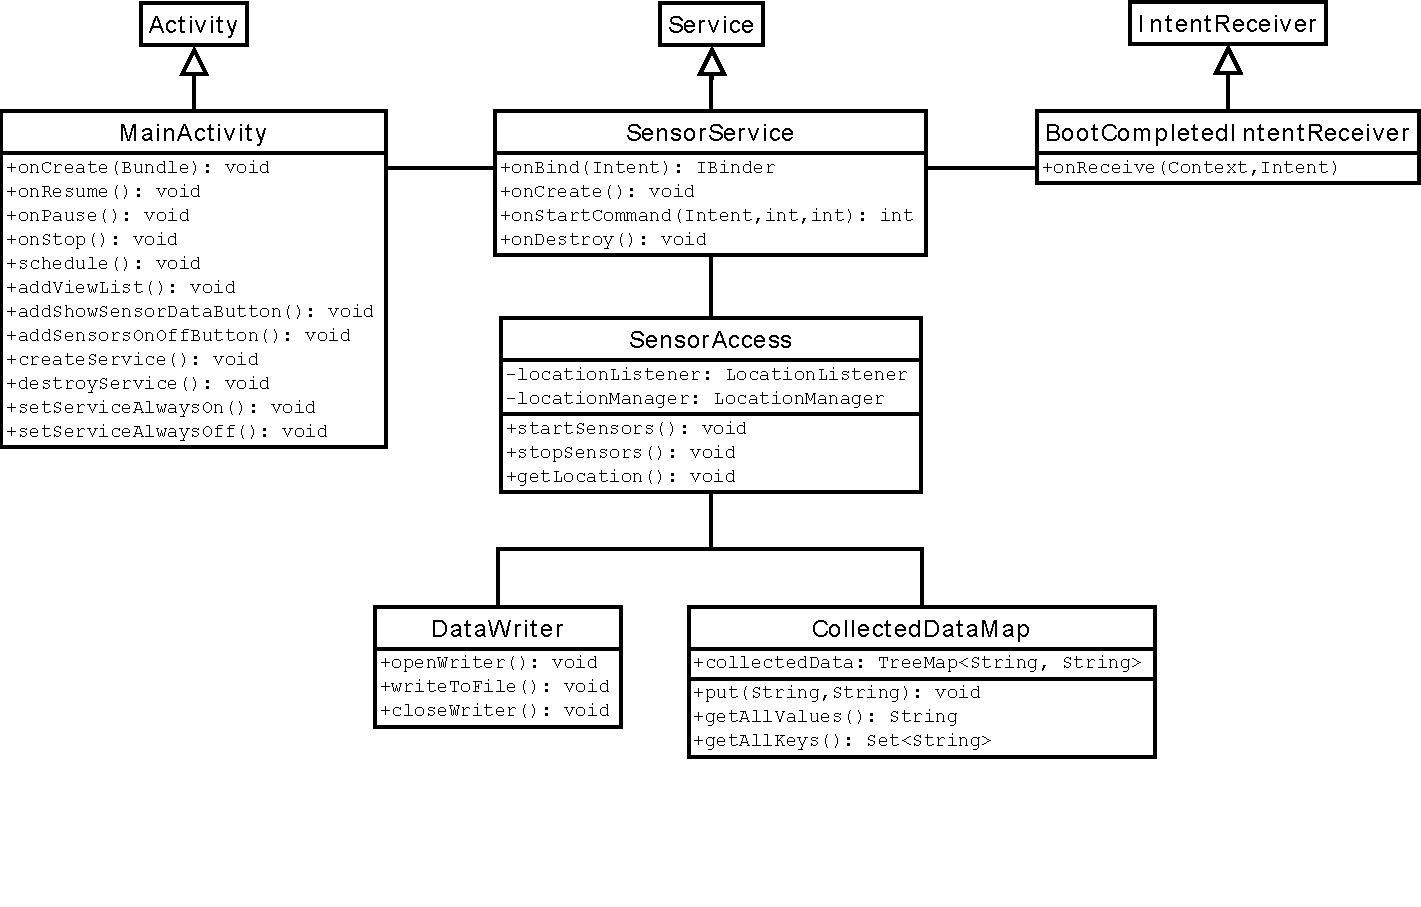
\includegraphics[height=70mm]{class_diagram.pdf}
% Lebenszyklus einzelner Komponenten ansprechen
\end{figure}
\end{frame}

\begin{frame}{Benutzeroberfl�che}
\begin{figure}[h]
\centering
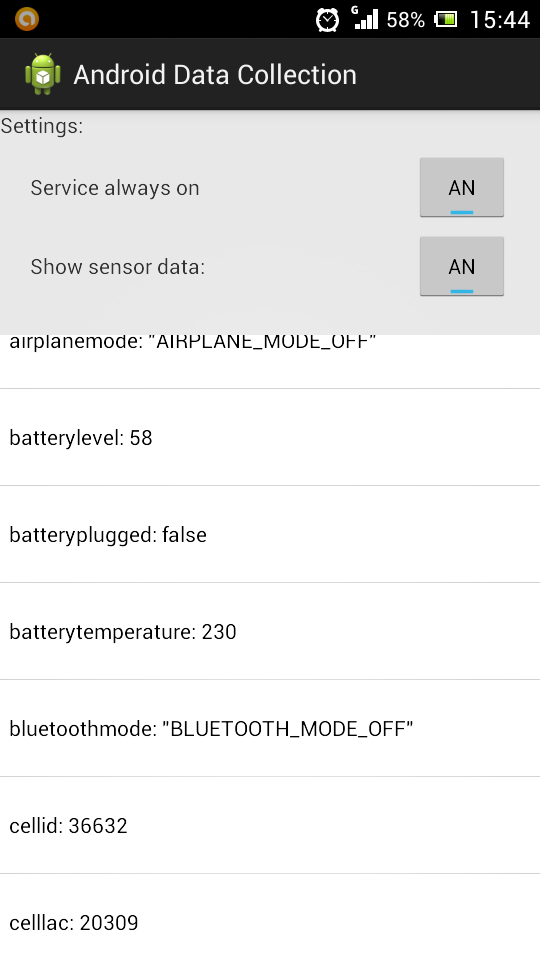
\includegraphics[height=70mm]{ui.png}
\end{figure}
\end{frame}

\begin{frame}{AndroidManifest}
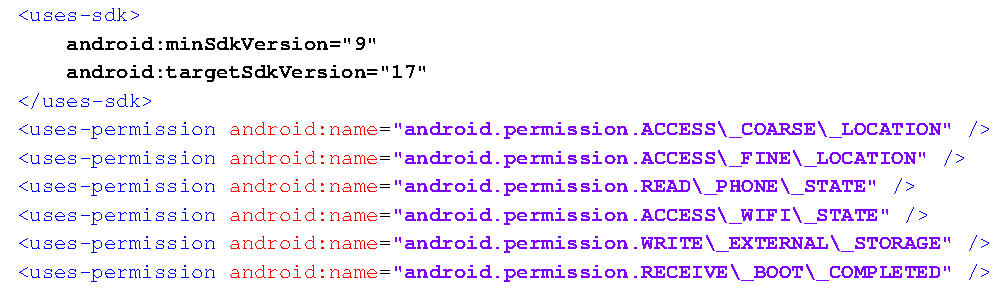
\includegraphics[width=1\linewidth]{android_manifest_cropped.pdf}
\end{frame}

%\begin{frame}{MainActivity}
%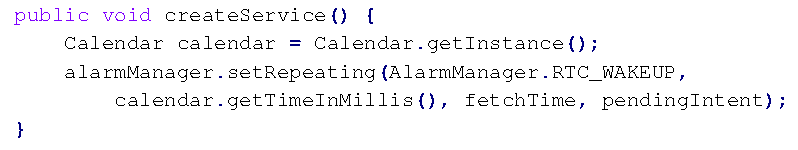
\includegraphics[width=1\linewidth]{createService_cropped.pdf}
%\end{frame}

%\begin{frame}{SensorService}
%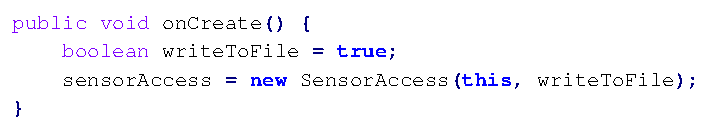
\includegraphics[width=1\linewidth]{onCreate_cropped.pdf}
%\end{frame}

%\begin{frame}{SensorService}
%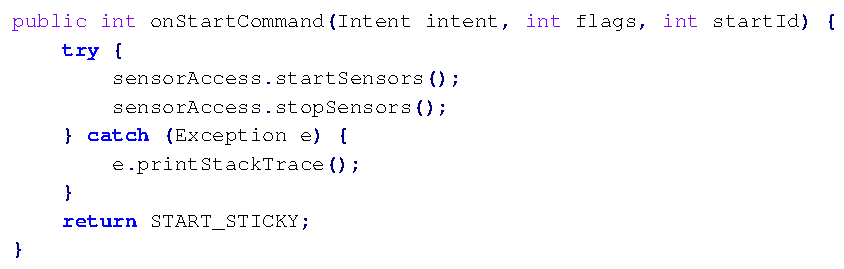
\includegraphics[width=1\linewidth]{onStartCommand_cropped.pdf}
%\end{frame}

\begin{frame}{SensorAccess}
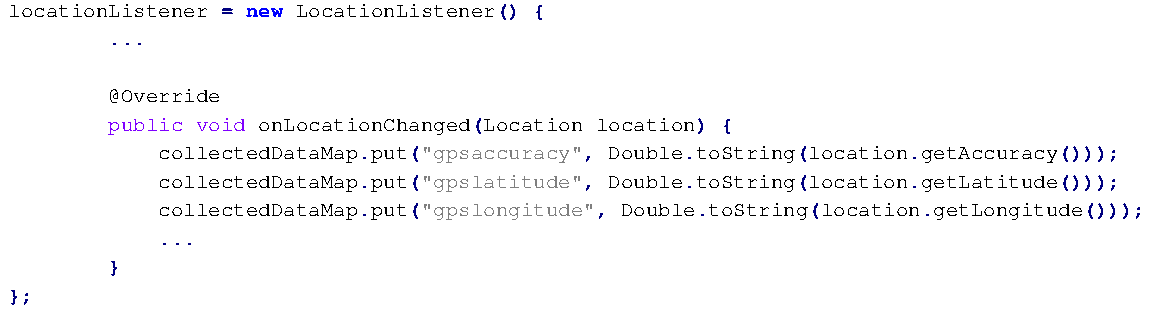
\includegraphics[width=1\linewidth]{getLocation_cropped.pdf}
\end{frame}

%\begin{frame}{BootCompletedIntentReceiver}
%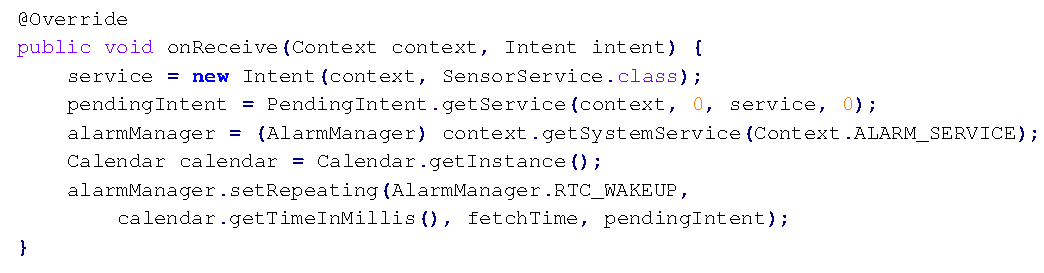
\includegraphics[width=1\linewidth]{onReceive_cropped.pdf}
%\end{frame}


\section{Bewegungsvorhersage}
\frame{\frametitle{Gliederung} \tableofcontents[currentsection]}

\begin{frame}{Modellierung}
\begin{itemize}
\item Nutzer bewegt sich durch die Stadt und �ndert seine Position
\end{itemize}

\begin{itemize}
\item Modellierung einer Bewegung als stochastischer Prozess
	\begin{itemize}
	\item Nutzer $u$ hat zum Zeitpunkt $t$ eine Position $x_t \in S$
	\item Beobachtungszeitraum $T = t_0, \ldots, t_n$
	\item Zustandsraum $S$ $\mathrel{\widehat{=}}$ Menge der Mobilfunkzellen
	\item Bewegung ist diskrete Zustands�nderung
	\end{itemize}
\end{itemize}

\vspace*{1em}

\begin{center}
\scalebox{.7}{%
% Graphic for TeX using PGF
% Title: C:\Users\Frank\Documents\1A Uni\1B Master\WS 1213\AndroidApp\AndroidDataCollection\Presentation\img\moving_user.dia
% Creator: Dia v0.97.1
% CreationDate: Sun Jun 30 13:07:57 2013
% For: Frank
% \usepackage{tikz}
% The following commands are not supported in PSTricks at present
% We define them conditionally, so when they are implemented,
% this pgf file will use them.
\ifx\du\undefined
  \newlength{\du}
\fi
\setlength{\du}{15\unitlength}
\begin{tikzpicture}
\pgftransformxscale{1.000000}
\pgftransformyscale{-1.000000}
\definecolor{dialinecolor}{rgb}{0.000000, 0.000000, 0.000000}
\pgfsetstrokecolor{dialinecolor}
\definecolor{dialinecolor}{rgb}{1.000000, 1.000000, 1.000000}
\pgfsetfillcolor{dialinecolor}
\pgfsetlinewidth{0.100000\du}
\pgfsetdash{}{0pt}
\pgfsetdash{}{0pt}
\pgfsetbuttcap
\pgfsetmiterjoin
\pgfsetlinewidth{0.100000\du}
\pgfsetbuttcap
\pgfsetmiterjoin
\pgfsetdash{}{0pt}
\definecolor{dialinecolor}{rgb}{0.466667, 0.466667, 0.466667}
\pgfsetfillcolor{dialinecolor}
\pgfpathellipse{\pgfpoint{16.500000\du}{1.500000\du}}{\pgfpoint{0.500000\du}{0\du}}{\pgfpoint{0\du}{0.500000\du}}
\pgfusepath{fill}
\definecolor{dialinecolor}{rgb}{0.000000, 0.000000, 0.000000}
\pgfsetstrokecolor{dialinecolor}
\pgfpathellipse{\pgfpoint{16.500000\du}{1.500000\du}}{\pgfpoint{0.500000\du}{0\du}}{\pgfpoint{0\du}{0.500000\du}}
\pgfusepath{stroke}
\pgfsetbuttcap
\pgfsetmiterjoin
\pgfsetdash{}{0pt}
\definecolor{dialinecolor}{rgb}{0.000000, 0.000000, 0.000000}
\pgfsetstrokecolor{dialinecolor}
\pgfpathellipse{\pgfpoint{16.500000\du}{1.500000\du}}{\pgfpoint{0.500000\du}{0\du}}{\pgfpoint{0\du}{0.500000\du}}
\pgfusepath{stroke}
\pgfsetlinewidth{0.100000\du}
\pgfsetdash{}{0pt}
\pgfsetdash{}{0pt}
\pgfsetbuttcap
\pgfsetmiterjoin
\pgfsetlinewidth{0.100000\du}
\pgfsetbuttcap
\pgfsetmiterjoin
\pgfsetdash{}{0pt}
\definecolor{dialinecolor}{rgb}{0.466667, 0.466667, 0.466667}
\pgfsetfillcolor{dialinecolor}
\pgfpathellipse{\pgfpoint{26.500000\du}{-2.500000\du}}{\pgfpoint{0.500000\du}{0\du}}{\pgfpoint{0\du}{0.500000\du}}
\pgfusepath{fill}
\definecolor{dialinecolor}{rgb}{0.000000, 0.000000, 0.000000}
\pgfsetstrokecolor{dialinecolor}
\pgfpathellipse{\pgfpoint{26.500000\du}{-2.500000\du}}{\pgfpoint{0.500000\du}{0\du}}{\pgfpoint{0\du}{0.500000\du}}
\pgfusepath{stroke}
\pgfsetbuttcap
\pgfsetmiterjoin
\pgfsetdash{}{0pt}
\definecolor{dialinecolor}{rgb}{0.000000, 0.000000, 0.000000}
\pgfsetstrokecolor{dialinecolor}
\pgfpathellipse{\pgfpoint{26.500000\du}{-2.500000\du}}{\pgfpoint{0.500000\du}{0\du}}{\pgfpoint{0\du}{0.500000\du}}
\pgfusepath{stroke}
\pgfsetlinewidth{0.100000\du}
\pgfsetdash{}{0pt}
\pgfsetdash{}{0pt}
\pgfsetbuttcap
\pgfsetmiterjoin
\pgfsetlinewidth{0.100000\du}
\pgfsetbuttcap
\pgfsetmiterjoin
\pgfsetdash{}{0pt}
\definecolor{dialinecolor}{rgb}{0.466667, 0.466667, 0.466667}
\pgfsetfillcolor{dialinecolor}
\pgfpathellipse{\pgfpoint{31.200000\du}{3.650000\du}}{\pgfpoint{0.500000\du}{0\du}}{\pgfpoint{0\du}{0.500000\du}}
\pgfusepath{fill}
\definecolor{dialinecolor}{rgb}{0.000000, 0.000000, 0.000000}
\pgfsetstrokecolor{dialinecolor}
\pgfpathellipse{\pgfpoint{31.200000\du}{3.650000\du}}{\pgfpoint{0.500000\du}{0\du}}{\pgfpoint{0\du}{0.500000\du}}
\pgfusepath{stroke}
\pgfsetbuttcap
\pgfsetmiterjoin
\pgfsetdash{}{0pt}
\definecolor{dialinecolor}{rgb}{0.000000, 0.000000, 0.000000}
\pgfsetstrokecolor{dialinecolor}
\pgfpathellipse{\pgfpoint{31.200000\du}{3.650000\du}}{\pgfpoint{0.500000\du}{0\du}}{\pgfpoint{0\du}{0.500000\du}}
\pgfusepath{stroke}
\pgfsetlinewidth{0.100000\du}
\pgfsetdash{}{0pt}
\pgfsetdash{}{0pt}
\pgfsetbuttcap
\pgfsetmiterjoin
\pgfsetlinewidth{0.100000\du}
\pgfsetbuttcap
\pgfsetmiterjoin
\pgfsetdash{}{0pt}
\definecolor{dialinecolor}{rgb}{0.466667, 0.466667, 0.466667}
\pgfsetfillcolor{dialinecolor}
\pgfpathellipse{\pgfpoint{39.250000\du}{0.500000\du}}{\pgfpoint{0.500000\du}{0\du}}{\pgfpoint{0\du}{0.500000\du}}
\pgfusepath{fill}
\definecolor{dialinecolor}{rgb}{0.000000, 0.000000, 0.000000}
\pgfsetstrokecolor{dialinecolor}
\pgfpathellipse{\pgfpoint{39.250000\du}{0.500000\du}}{\pgfpoint{0.500000\du}{0\du}}{\pgfpoint{0\du}{0.500000\du}}
\pgfusepath{stroke}
\pgfsetbuttcap
\pgfsetmiterjoin
\pgfsetdash{}{0pt}
\definecolor{dialinecolor}{rgb}{0.000000, 0.000000, 0.000000}
\pgfsetstrokecolor{dialinecolor}
\pgfpathellipse{\pgfpoint{39.250000\du}{0.500000\du}}{\pgfpoint{0.500000\du}{0\du}}{\pgfpoint{0\du}{0.500000\du}}
\pgfusepath{stroke}
\pgfsetlinewidth{0.100000\du}
\pgfsetdash{}{0pt}
\pgfsetdash{}{0pt}
\pgfsetbuttcap
{
\definecolor{dialinecolor}{rgb}{0.000000, 0.000000, 0.000000}
\pgfsetfillcolor{dialinecolor}
% was here!!!
\pgfsetarrowsend{to}
\definecolor{dialinecolor}{rgb}{0.000000, 0.000000, 0.000000}
\pgfsetstrokecolor{dialinecolor}
\draw (17.010864\du,1.295654\du)--(25.989136\du,-2.295654\du);
}
\pgfsetlinewidth{0.100000\du}
\pgfsetdash{}{0pt}
\pgfsetdash{}{0pt}
\pgfsetbuttcap
{
\definecolor{dialinecolor}{rgb}{0.000000, 0.000000, 0.000000}
\pgfsetfillcolor{dialinecolor}
% was here!!!
\pgfsetarrowsend{to}
\definecolor{dialinecolor}{rgb}{0.000000, 0.000000, 0.000000}
\pgfsetstrokecolor{dialinecolor}
\draw (26.834198\du,-2.062698\du)--(30.865802\du,3.212698\du);
}
\pgfsetlinewidth{0.100000\du}
\pgfsetdash{}{0pt}
\pgfsetdash{}{0pt}
\pgfsetbuttcap
{
\definecolor{dialinecolor}{rgb}{0.000000, 0.000000, 0.000000}
\pgfsetfillcolor{dialinecolor}
% was here!!!
\pgfsetarrowsend{to}
\definecolor{dialinecolor}{rgb}{0.000000, 0.000000, 0.000000}
\pgfsetstrokecolor{dialinecolor}
\draw (31.711969\du,3.449664\du)--(38.738031\du,0.700336\du);
}
\pgfsetlinewidth{0.100000\du}
\pgfsetdash{}{0pt}
\pgfsetdash{}{0pt}
\pgfsetbuttcap
\pgfsetmiterjoin
\pgfsetlinewidth{0.100000\du}
\pgfsetbuttcap
\pgfsetmiterjoin
\pgfsetdash{}{0pt}
\definecolor{dialinecolor}{rgb}{0.466667, 0.466667, 0.466667}
\pgfsetfillcolor{dialinecolor}
\pgfpathellipse{\pgfpoint{23.665100\du}{0.842500\du}}{\pgfpoint{0.500000\du}{0\du}}{\pgfpoint{0\du}{0.500000\du}}
\pgfusepath{fill}
\definecolor{dialinecolor}{rgb}{0.000000, 0.000000, 0.000000}
\pgfsetstrokecolor{dialinecolor}
\pgfpathellipse{\pgfpoint{23.665100\du}{0.842500\du}}{\pgfpoint{0.500000\du}{0\du}}{\pgfpoint{0\du}{0.500000\du}}
\pgfusepath{stroke}
\pgfsetbuttcap
\pgfsetmiterjoin
\pgfsetdash{}{0pt}
\definecolor{dialinecolor}{rgb}{0.000000, 0.000000, 0.000000}
\pgfsetstrokecolor{dialinecolor}
\pgfpathellipse{\pgfpoint{23.665100\du}{0.842500\du}}{\pgfpoint{0.500000\du}{0\du}}{\pgfpoint{0\du}{0.500000\du}}
\pgfusepath{stroke}
\pgfsetlinewidth{0.100000\du}
\pgfsetdash{}{0pt}
\pgfsetdash{}{0pt}
\pgfsetbuttcap
{
\definecolor{dialinecolor}{rgb}{0.000000, 0.000000, 0.000000}
\pgfsetfillcolor{dialinecolor}
% was here!!!
\pgfsetarrowsend{to}
\definecolor{dialinecolor}{rgb}{0.000000, 0.000000, 0.000000}
\pgfsetstrokecolor{dialinecolor}
\draw (38.699715\du,0.512093\du)--(24.215385\du,0.830407\du);
}
\end{tikzpicture}

}
\end{center}
\end{frame}

\begin{frame}{Markov Modelle - Transitionsdiagramm}
\begin{itemize}
\item Zustandsraum $S = 1, \ldots, m$
\item Zustands�nderungen als Transitionsdiagramm
\item �bergangswahrscheinlichkeiten in Transitionsmatrix $A$
	\begin{itemize}
	\item[$\Rightarrow$] Annahme: station�re\\ �bergangswahrscheinlichkeiten
	\end{itemize}
\end{itemize}

\vspace*{-2.5em}
\begin{columns}
\column{0.5\textwidth}
$$A=\begin{bmatrix}
A_{11} & A_{12} & A_{13} \\
A_{21} & A_{22} & A_{23} \\
A_{31} & A_{32} & A_{33}
\end{bmatrix}$$
\begin{align*}
A_{ij} &\geq 0\\ %nichtnegativ
\sum\limits_{j \in S} A_{ij} &= 1 %Zeilensumme = 1
\end{align*}
\vspace*{-4em}

\column{0.5\textwidth}
\begin{center}
\scalebox{.3}{%
\scalefont{2}
% Graphic for TeX using PGF
% Title: C:\Users\Frank\Documents\1A Uni\1B Master\WS 1213\AndroidApp\AndroidDataCollection\Presentation\img\transition_chart
% Creator: Dia v0.97.1
% CreationDate: Sun Jun 30 14:26:08 2013
% For: Frank
% \usepackage{tikz}
% The following commands are not supported in PSTricks at present
% We define them conditionally, so when they are implemented,
% this pgf file will use them.
\ifx\du\undefined
  \newlength{\du}
\fi
\setlength{\du}{15\unitlength}
\begin{tikzpicture}
\pgftransformxscale{1.000000}
\pgftransformyscale{-1.000000}
\definecolor{dialinecolor}{rgb}{0.000000, 0.000000, 0.000000}
\pgfsetstrokecolor{dialinecolor}
\definecolor{dialinecolor}{rgb}{1.000000, 1.000000, 1.000000}
\pgfsetfillcolor{dialinecolor}
\pgfsetlinewidth{0.500000\du}
\pgfsetdash{}{0pt}
\pgfsetdash{}{0pt}
\pgfsetroundjoin
{\pgfsetcornersarced{\pgfpoint{0.500000\du}{0.500000\du}}\definecolor{dialinecolor}{rgb}{1.000000, 1.000000, 1.000000}
\pgfsetfillcolor{dialinecolor}
\fill (19.000000\du,17.000000\du)--(19.000000\du,20.000000\du)--(22.000000\du,20.000000\du)--(22.000000\du,17.000000\du)--cycle;
}{\pgfsetcornersarced{\pgfpoint{0.500000\du}{0.500000\du}}\definecolor{dialinecolor}{rgb}{0.000000, 0.000000, 1.000000}
\pgfsetstrokecolor{dialinecolor}
\draw (19.000000\du,17.000000\du)--(19.000000\du,20.000000\du)--(22.000000\du,20.000000\du)--(22.000000\du,17.000000\du)--cycle;
}\pgfsetlinewidth{0.500000\du}
\pgfsetdash{}{0pt}
\pgfsetdash{}{0pt}
\pgfsetroundjoin
{\pgfsetcornersarced{\pgfpoint{0.500000\du}{0.500000\du}}\definecolor{dialinecolor}{rgb}{1.000000, 1.000000, 1.000000}
\pgfsetfillcolor{dialinecolor}
\fill (28.146447\du,10.146447\du)--(28.146447\du,12.853553\du)--(30.853553\du,12.853553\du)--(30.853553\du,10.146447\du)--cycle;
}{\pgfsetcornersarced{\pgfpoint{0.500000\du}{0.500000\du}}\definecolor{dialinecolor}{rgb}{0.717647, 0.000000, 0.000000}
\pgfsetstrokecolor{dialinecolor}
\draw (28.146447\du,10.146447\du)--(28.146447\du,12.853553\du)--(30.853553\du,12.853553\du)--(30.853553\du,10.146447\du)--cycle;
}\pgfsetlinewidth{0.500000\du}
\pgfsetdash{}{0pt}
\pgfsetdash{}{0pt}
\pgfsetroundjoin
{\pgfsetcornersarced{\pgfpoint{0.500000\du}{0.500000\du}}\definecolor{dialinecolor}{rgb}{1.000000, 1.000000, 1.000000}
\pgfsetfillcolor{dialinecolor}
\fill (19.000000\du,3.000000\du)--(19.000000\du,6.000000\du)--(22.000000\du,6.000000\du)--(22.000000\du,3.000000\du)--cycle;
}{\pgfsetcornersarced{\pgfpoint{0.500000\du}{0.500000\du}}\definecolor{dialinecolor}{rgb}{0.000000, 0.509804, 0.000000}
\pgfsetstrokecolor{dialinecolor}
\draw (19.000000\du,3.000000\du)--(19.000000\du,6.000000\du)--(22.000000\du,6.000000\du)--(22.000000\du,3.000000\du)--cycle;
}% setfont left to latex
\definecolor{dialinecolor}{rgb}{0.717647, 0.000000, 0.000000}
\pgfsetstrokecolor{dialinecolor}
\node[anchor=east] at (28.146447\du,11.823469\du){$\color{dialinecolor}{x = 1}$  };
% setfont left to latex
\definecolor{dialinecolor}{rgb}{0.000000, 0.000000, 1.000000}
\pgfsetstrokecolor{dialinecolor}
\node at (20.500000\du,15.873875\du){$\color{dialinecolor}{x = 2}$};
% setfont left to latex
\definecolor{dialinecolor}{rgb}{0.000000, 0.509804, 0.000000}
\pgfsetstrokecolor{dialinecolor}
\node at (20.500000\du,7\du){$\color{dialinecolor}{x = 3}$};
\pgfsetlinewidth{0.100000\du}
\pgfsetdash{}{0pt}
\pgfsetdash{}{0pt}
\pgfsetbuttcap
{
\definecolor{dialinecolor}{rgb}{0.000000, 0.000000, 0.000000}
\pgfsetfillcolor{dialinecolor}
% was here!!!
\pgfsetarrowsend{to}
\definecolor{dialinecolor}{rgb}{0.000000, 0.000000, 0.000000}
\pgfsetstrokecolor{dialinecolor}
\pgfpathmoveto{\pgfpoint{31.499882\du}{12.999905\du}}
\pgfpatharc{129}{-128}{2.243153\du and 2.243153\du}
\pgfusepath{stroke}
}
\pgfsetlinewidth{0.100000\du}
\pgfsetdash{}{0pt}
\pgfsetdash{}{0pt}
\pgfsetbuttcap
{
\definecolor{dialinecolor}{rgb}{0.000000, 0.000000, 0.000000}
\pgfsetfillcolor{dialinecolor}
% was here!!!
\pgfsetarrowsend{to}
\definecolor{dialinecolor}{rgb}{0.000000, 0.000000, 0.000000}
\pgfsetstrokecolor{dialinecolor}
\pgfpathmoveto{\pgfpoint{18.500055\du}{20.499914\du}}
\pgfpatharc{213}{-32}{2.371702\du and 2.371702\du}
\pgfusepath{stroke}
}
\pgfsetlinewidth{0.100000\du}
\pgfsetdash{}{0pt}
\pgfsetdash{}{0pt}
\pgfsetbuttcap
{
\definecolor{dialinecolor}{rgb}{0.000000, 0.000000, 0.000000}
\pgfsetfillcolor{dialinecolor}
% was here!!!
\pgfsetarrowsend{to}
\definecolor{dialinecolor}{rgb}{0.000000, 0.000000, 0.000000}
\pgfsetstrokecolor{dialinecolor}
\pgfpathmoveto{\pgfpoint{22.499878\du}{2.500192\du}}
\pgfpatharc{33}{-212}{2.371702\du and 2.371702\du}
\pgfusepath{stroke}
}
\pgfsetlinewidth{0.100000\du}
\pgfsetdash{}{0pt}
\pgfsetdash{}{0pt}
\pgfsetbuttcap
{
\definecolor{dialinecolor}{rgb}{0.000000, 0.000000, 0.000000}
\pgfsetfillcolor{dialinecolor}
% was here!!!
\pgfsetarrowsend{to}
\definecolor{dialinecolor}{rgb}{0.000000, 0.000000, 0.000000}
\pgfsetstrokecolor{dialinecolor}
\pgfpathmoveto{\pgfpoint{30.000013\du}{9.000038\du}}
\pgfpatharc{341}{269}{7.152814\du and 7.152814\du}
\pgfusepath{stroke}
}
\pgfsetlinewidth{0.100000\du}
\pgfsetdash{}{0pt}
\pgfsetdash{}{0pt}
\pgfsetbuttcap
{
\definecolor{dialinecolor}{rgb}{0.000000, 0.000000, 0.000000}
\pgfsetfillcolor{dialinecolor}
% was here!!!
\pgfsetarrowsend{to}
\definecolor{dialinecolor}{rgb}{0.000000, 0.000000, 0.000000}
\pgfsetstrokecolor{dialinecolor}
\pgfpathmoveto{\pgfpoint{18.000222\du}{4.999888\du}}
\pgfpatharc{244}{117}{7.281250\du and 7.281250\du}
\pgfusepath{stroke}
}
\pgfsetlinewidth{0.100000\du}
\pgfsetdash{}{0pt}
\pgfsetdash{}{0pt}
\pgfsetbuttcap
{
\definecolor{dialinecolor}{rgb}{0.000000, 0.000000, 0.000000}
\pgfsetfillcolor{dialinecolor}
% was here!!!
\pgfsetarrowsend{to}
\definecolor{dialinecolor}{rgb}{0.000000, 0.000000, 0.000000}
\pgfsetstrokecolor{dialinecolor}
\pgfpathmoveto{\pgfpoint{22.999408\du}{19.000005\du}}
\pgfpatharc{90}{20}{7.481032\du and 7.481032\du}
\pgfusepath{stroke}
}
\pgfsetlinewidth{0.100000\du}
\pgfsetdash{}{0pt}
\pgfsetdash{}{0pt}
\pgfsetmiterjoin
\pgfsetbuttcap
{
\definecolor{dialinecolor}{rgb}{0.000000, 0.000000, 0.000000}
\pgfsetfillcolor{dialinecolor}
% was here!!!
\pgfsetarrowsend{to}
\definecolor{dialinecolor}{rgb}{0.000000, 0.000000, 0.000000}
\pgfsetstrokecolor{dialinecolor}
\pgfpathmoveto{\pgfpoint{18.000000\du}{17.000000\du}}
\pgfpathcurveto{\pgfpoint{14.000000\du}{14.500000\du}}{\pgfpoint{14.000000\du}{8.500000\du}}{\pgfpoint{18.000000\du}{6.000000\du}}
\pgfusepath{stroke}
}
\pgfsetlinewidth{0.100000\du}
\pgfsetdash{}{0pt}
\pgfsetdash{}{0pt}
\pgfsetmiterjoin
\pgfsetbuttcap
{
\definecolor{dialinecolor}{rgb}{0.000000, 0.000000, 0.000000}
\pgfsetfillcolor{dialinecolor}
% was here!!!
\pgfsetarrowsend{to}
\definecolor{dialinecolor}{rgb}{0.000000, 0.000000, 0.000000}
\pgfsetstrokecolor{dialinecolor}
\pgfpathmoveto{\pgfpoint{23.000000\du}{5.200000\du}}
\pgfpathcurveto{\pgfpoint{25.500000\du}{5.200000\du}}{\pgfpoint{28.000000\du}{6.600000\du}}{\pgfpoint{29.000000\du}{9.000000\du}}
\pgfusepath{stroke}
}
\pgfsetlinewidth{0.100000\du}
\pgfsetdash{}{0pt}
\pgfsetdash{}{0pt}
\pgfsetmiterjoin
\pgfsetbuttcap
{
\definecolor{dialinecolor}{rgb}{0.000000, 0.000000, 0.000000}
\pgfsetfillcolor{dialinecolor}
% was here!!!
\pgfsetarrowsend{to}
\definecolor{dialinecolor}{rgb}{0.000000, 0.000000, 0.000000}
\pgfsetstrokecolor{dialinecolor}
\pgfpathmoveto{\pgfpoint{29.000000\du}{14.000000\du}}
\pgfpathcurveto{\pgfpoint{27.900000\du}{16.300000\du}}{\pgfpoint{25.800000\du}{17.700000\du}}{\pgfpoint{23.000000\du}{18.000000\du}}
\pgfusepath{stroke}
}
% setfont left to latex
\definecolor{dialinecolor}{rgb}{0.000000, 0.000000, 0.000000}
\pgfsetstrokecolor{dialinecolor}
\node at (29.050000\du,4.844094\du){$A_{13}$};
% setfont left to latex
\definecolor{dialinecolor}{rgb}{0.000000, 0.000000, 0.000000}
\pgfsetstrokecolor{dialinecolor}
\node at (25.394219\du,7.317375\du){$A_{31}$};
% setfont left to latex
\definecolor{dialinecolor}{rgb}{0.000000, 0.000000, 0.000000}
\pgfsetstrokecolor{dialinecolor}
\node at (28.449219\du,18.622375\du){$A_{21}$};
% setfont left to latex
\definecolor{dialinecolor}{rgb}{0.000000, 0.000000, 0.000000}
\pgfsetstrokecolor{dialinecolor}
\node at (25.604219\du,15.877375\du){$A_{12}$};
% setfont left to latex
\definecolor{dialinecolor}{rgb}{0.000000, 0.000000, 0.000000}
\pgfsetstrokecolor{dialinecolor}
\node at (17.000000\du,11.753750\du){$A_{23}$};
% setfont left to latex
\definecolor{dialinecolor}{rgb}{0.000000, 0.000000, 0.000000}
\pgfsetstrokecolor{dialinecolor}
\node at (12.000000\du,11.753750\du){$A_{32}$};
% setfont left to latex
\definecolor{dialinecolor}{rgb}{0.000000, 0.000000, 0.000000}
\pgfsetstrokecolor{dialinecolor}
\node at (16.251719\du,1.249531\du){$A_{33}$};
% setfont left to latex
\definecolor{dialinecolor}{rgb}{0.000000, 0.000000, 0.000000}
\pgfsetstrokecolor{dialinecolor}
\node at (36.856719\du,11.504531\du){$A_{11}$};
% setfont left to latex
\definecolor{dialinecolor}{rgb}{0.000000, 0.000000, 0.000000}
\pgfsetstrokecolor{dialinecolor}
\node at (16.261719\du,22.359531\du){$A_{22}$};
\end{tikzpicture}

}
\end{center}
\vspace*{.5em}
\hfill \tiny Vgl. \cite{bishop2006pattern}, S.~611 \hspace*{4em}
\end{columns}

\end{frame}

\begin{frame}{Markov Modelle - Grafisches Modell}
\begin{itemize}
\item Zustandsraum $S = 1, \ldots, m$, Zeitreihe $T = t_0, t_1, \ldots$
\item Zustands�nderungen als graphisches Modell
\end{itemize}
\begin{center}
\scalebox{.6}{%
\scalefont{2}
% Graphic for TeX using PGF
% Title: C:\Users\Frank\Documents\1A Uni\1B Master\WS 1213\AndroidApp\AndroidDataCollection\WriteUpFrank\img\graphical_model.dia
% Creator: Dia v0.97.1
% CreationDate: Mon Sep 09 10:46:57 2013
% For: Frank
% \usepackage{tikz}
% The following commands are not supported in PSTricks at present
% We define them conditionally, so when they are implemented,
% this pgf file will use them.
\ifx\du\undefined
  \newlength{\du}
\fi
\setlength{\du}{15\unitlength}
\begin{tikzpicture}
\pgftransformxscale{1.000000}
\pgftransformyscale{-1.000000}
\definecolor{dialinecolor}{rgb}{0.000000, 0.000000, 0.000000}
\pgfsetstrokecolor{dialinecolor}
\definecolor{dialinecolor}{rgb}{1.000000, 1.000000, 1.000000}
\pgfsetfillcolor{dialinecolor}
\pgfsetlinewidth{0.100000\du}
\pgfsetdash{}{0pt}
\pgfsetdash{}{0pt}
\pgfsetbuttcap
\pgfsetmiterjoin
\pgfsetlinewidth{0.100000\du}
\pgfsetbuttcap
\pgfsetmiterjoin
\pgfsetdash{}{0pt}
\definecolor{dialinecolor}{rgb}{0.823529, 0.823529, 0.823529}
\pgfsetfillcolor{dialinecolor}
\pgfpathellipse{\pgfpoint{21.000000\du}{17.000000\du}}{\pgfpoint{1.000000\du}{0\du}}{\pgfpoint{0\du}{1.000000\du}}
\pgfusepath{fill}
\definecolor{dialinecolor}{rgb}{0.000000, 0.000000, 0.000000}
\pgfsetstrokecolor{dialinecolor}
\pgfpathellipse{\pgfpoint{21.000000\du}{17.000000\du}}{\pgfpoint{1.000000\du}{0\du}}{\pgfpoint{0\du}{1.000000\du}}
\pgfusepath{stroke}
\pgfsetbuttcap
\pgfsetmiterjoin
\pgfsetdash{}{0pt}
\definecolor{dialinecolor}{rgb}{0.000000, 0.000000, 0.000000}
\pgfsetstrokecolor{dialinecolor}
\pgfpathellipse{\pgfpoint{21.000000\du}{17.000000\du}}{\pgfpoint{1.000000\du}{0\du}}{\pgfpoint{0\du}{1.000000\du}}
\pgfusepath{stroke}
\pgfsetlinewidth{0.100000\du}
\pgfsetdash{}{0pt}
\pgfsetdash{}{0pt}
\pgfsetbuttcap
{
\definecolor{dialinecolor}{rgb}{0.000000, 0.000000, 0.000000}
\pgfsetfillcolor{dialinecolor}
% was here!!!
\pgfsetarrowsend{to}
\definecolor{dialinecolor}{rgb}{0.000000, 0.000000, 0.000000}
\pgfsetstrokecolor{dialinecolor}
\draw (22.000000\du,17.000000\du)--(24.000000\du,17.000000\du);
}
\pgfsetlinewidth{0.100000\du}
\pgfsetdash{}{0pt}
\pgfsetdash{}{0pt}
\pgfsetbuttcap
\pgfsetmiterjoin
\pgfsetlinewidth{0.100000\du}
\pgfsetbuttcap
\pgfsetmiterjoin
\pgfsetdash{}{0pt}
\definecolor{dialinecolor}{rgb}{0.823529, 0.823529, 0.823529}
\pgfsetfillcolor{dialinecolor}
\pgfpathellipse{\pgfpoint{25.000000\du}{17.000000\du}}{\pgfpoint{1.000000\du}{0\du}}{\pgfpoint{0\du}{1.000000\du}}
\pgfusepath{fill}
\definecolor{dialinecolor}{rgb}{0.000000, 0.000000, 0.000000}
\pgfsetstrokecolor{dialinecolor}
\pgfpathellipse{\pgfpoint{25.000000\du}{17.000000\du}}{\pgfpoint{1.000000\du}{0\du}}{\pgfpoint{0\du}{1.000000\du}}
\pgfusepath{stroke}
\pgfsetbuttcap
\pgfsetmiterjoin
\pgfsetdash{}{0pt}
\definecolor{dialinecolor}{rgb}{0.000000, 0.000000, 0.000000}
\pgfsetstrokecolor{dialinecolor}
\pgfpathellipse{\pgfpoint{25.000000\du}{17.000000\du}}{\pgfpoint{1.000000\du}{0\du}}{\pgfpoint{0\du}{1.000000\du}}
\pgfusepath{stroke}
\pgfsetlinewidth{0.100000\du}
\pgfsetdash{}{0pt}
\pgfsetdash{}{0pt}
\pgfsetbuttcap
{
\definecolor{dialinecolor}{rgb}{0.000000, 0.000000, 0.000000}
\pgfsetfillcolor{dialinecolor}
% was here!!!
\pgfsetarrowsend{to}
\definecolor{dialinecolor}{rgb}{0.000000, 0.000000, 0.000000}
\pgfsetstrokecolor{dialinecolor}
\draw (26.000000\du,17.000000\du)--(28.000000\du,17.000000\du);
}
\pgfsetlinewidth{0.100000\du}
\pgfsetdash{}{0pt}
\pgfsetdash{}{0pt}
\pgfsetbuttcap
\pgfsetmiterjoin
\pgfsetlinewidth{0.100000\du}
\pgfsetbuttcap
\pgfsetmiterjoin
\pgfsetdash{}{0pt}
\definecolor{dialinecolor}{rgb}{0.823529, 0.823529, 0.823529}
\pgfsetfillcolor{dialinecolor}
\pgfpathellipse{\pgfpoint{29.000000\du}{17.000000\du}}{\pgfpoint{1.000000\du}{0\du}}{\pgfpoint{0\du}{1.000000\du}}
\pgfusepath{fill}
\definecolor{dialinecolor}{rgb}{0.000000, 0.000000, 0.000000}
\pgfsetstrokecolor{dialinecolor}
\pgfpathellipse{\pgfpoint{29.000000\du}{17.000000\du}}{\pgfpoint{1.000000\du}{0\du}}{\pgfpoint{0\du}{1.000000\du}}
\pgfusepath{stroke}
\pgfsetbuttcap
\pgfsetmiterjoin
\pgfsetdash{}{0pt}
\definecolor{dialinecolor}{rgb}{0.000000, 0.000000, 0.000000}
\pgfsetstrokecolor{dialinecolor}
\pgfpathellipse{\pgfpoint{29.000000\du}{17.000000\du}}{\pgfpoint{1.000000\du}{0\du}}{\pgfpoint{0\du}{1.000000\du}}
\pgfusepath{stroke}
\pgfsetlinewidth{0.100000\du}
\pgfsetdash{}{0pt}
\pgfsetdash{}{0pt}
\pgfsetbuttcap
{
\definecolor{dialinecolor}{rgb}{0.000000, 0.000000, 0.000000}
\pgfsetfillcolor{dialinecolor}
% was here!!!
\pgfsetarrowsend{to}
\definecolor{dialinecolor}{rgb}{0.000000, 0.000000, 0.000000}
\pgfsetstrokecolor{dialinecolor}
\draw (30.000000\du,17.000000\du)--(32.000000\du,17.000000\du);
}
\pgfsetlinewidth{0.100000\du}
\pgfsetdash{}{0pt}
\pgfsetdash{}{0pt}
\pgfsetbuttcap
\pgfsetmiterjoin
\pgfsetlinewidth{0.100000\du}
\pgfsetbuttcap
\pgfsetmiterjoin
\pgfsetdash{}{0pt}
\definecolor{dialinecolor}{rgb}{0.823529, 0.823529, 0.823529}
\pgfsetfillcolor{dialinecolor}
\pgfpathellipse{\pgfpoint{41.000000\du}{17.000000\du}}{\pgfpoint{1.000000\du}{0\du}}{\pgfpoint{0\du}{1.000000\du}}
\pgfusepath{fill}
\definecolor{dialinecolor}{rgb}{0.000000, 0.000000, 0.000000}
\pgfsetstrokecolor{dialinecolor}
\pgfpathellipse{\pgfpoint{41.000000\du}{17.000000\du}}{\pgfpoint{1.000000\du}{0\du}}{\pgfpoint{0\du}{1.000000\du}}
\pgfusepath{stroke}
\pgfsetbuttcap
\pgfsetmiterjoin
\pgfsetdash{}{0pt}
\definecolor{dialinecolor}{rgb}{0.000000, 0.000000, 0.000000}
\pgfsetstrokecolor{dialinecolor}
\pgfpathellipse{\pgfpoint{41.000000\du}{17.000000\du}}{\pgfpoint{1.000000\du}{0\du}}{\pgfpoint{0\du}{1.000000\du}}
\pgfusepath{stroke}
\pgfsetlinewidth{0.100000\du}
\pgfsetdash{}{0pt}
\pgfsetdash{}{0pt}
\pgfsetbuttcap
{
\definecolor{dialinecolor}{rgb}{0.000000, 0.000000, 0.000000}
\pgfsetfillcolor{dialinecolor}
% was here!!!
\pgfsetarrowsend{to}
\definecolor{dialinecolor}{rgb}{0.000000, 0.000000, 0.000000}
\pgfsetstrokecolor{dialinecolor}
\draw (42.000000\du,17.000000\du)--(44.000000\du,17.000000\du);
}
\pgfsetlinewidth{0.100000\du}
\pgfsetdash{}{0pt}
\pgfsetdash{}{0pt}
\pgfsetbuttcap
\pgfsetmiterjoin
\pgfsetlinewidth{0.100000\du}
\pgfsetbuttcap
\pgfsetmiterjoin
\pgfsetdash{}{0pt}
\definecolor{dialinecolor}{rgb}{0.823529, 0.823529, 0.823529}
\pgfsetfillcolor{dialinecolor}
\pgfpathellipse{\pgfpoint{45.000000\du}{17.000000\du}}{\pgfpoint{1.000000\du}{0\du}}{\pgfpoint{0\du}{1.000000\du}}
\pgfusepath{fill}
\definecolor{dialinecolor}{rgb}{0.000000, 0.000000, 0.000000}
\pgfsetstrokecolor{dialinecolor}
\pgfpathellipse{\pgfpoint{45.000000\du}{17.000000\du}}{\pgfpoint{1.000000\du}{0\du}}{\pgfpoint{0\du}{1.000000\du}}
\pgfusepath{stroke}
\pgfsetbuttcap
\pgfsetmiterjoin
\pgfsetdash{}{0pt}
\definecolor{dialinecolor}{rgb}{0.000000, 0.000000, 0.000000}
\pgfsetstrokecolor{dialinecolor}
\pgfpathellipse{\pgfpoint{45.000000\du}{17.000000\du}}{\pgfpoint{1.000000\du}{0\du}}{\pgfpoint{0\du}{1.000000\du}}
\pgfusepath{stroke}
\pgfsetlinewidth{0.100000\du}
\pgfsetdash{}{0pt}
\pgfsetdash{}{0pt}
\pgfsetbuttcap
{
\definecolor{dialinecolor}{rgb}{0.000000, 0.000000, 0.000000}
\pgfsetfillcolor{dialinecolor}
% was here!!!
\pgfsetarrowsend{to}
\definecolor{dialinecolor}{rgb}{0.000000, 0.000000, 0.000000}
\pgfsetstrokecolor{dialinecolor}
\draw (46.000000\du,17.000000\du)--(48.000000\du,17.000000\du);
}
\pgfsetlinewidth{0.100000\du}
\pgfsetdash{}{0pt}
\pgfsetdash{}{0pt}
\pgfsetbuttcap
\pgfsetmiterjoin
\pgfsetlinewidth{0.100000\du}
\pgfsetbuttcap
\pgfsetmiterjoin
\pgfsetdash{}{0pt}
\definecolor{dialinecolor}{rgb}{0.000000, 0.000000, 0.000000}
\pgfsetfillcolor{dialinecolor}
\pgfpathellipse{\pgfpoint{49.096875\du}{16.996875\du}}{\pgfpoint{0.096875\du}{0\du}}{\pgfpoint{0\du}{0.096875\du}}
\pgfusepath{fill}
\definecolor{dialinecolor}{rgb}{0.000000, 0.000000, 0.000000}
\pgfsetstrokecolor{dialinecolor}
\pgfpathellipse{\pgfpoint{49.096875\du}{16.996875\du}}{\pgfpoint{0.096875\du}{0\du}}{\pgfpoint{0\du}{0.096875\du}}
\pgfusepath{stroke}
\pgfsetbuttcap
\pgfsetmiterjoin
\pgfsetdash{}{0pt}
\definecolor{dialinecolor}{rgb}{0.000000, 0.000000, 0.000000}
\pgfsetstrokecolor{dialinecolor}
\pgfpathellipse{\pgfpoint{49.096875\du}{16.996875\du}}{\pgfpoint{0.096875\du}{0\du}}{\pgfpoint{0\du}{0.096875\du}}
\pgfusepath{stroke}
\pgfsetlinewidth{0.100000\du}
\pgfsetdash{}{0pt}
\pgfsetdash{}{0pt}
\pgfsetbuttcap
\pgfsetmiterjoin
\pgfsetlinewidth{0.100000\du}
\pgfsetbuttcap
\pgfsetmiterjoin
\pgfsetdash{}{0pt}
\definecolor{dialinecolor}{rgb}{0.000000, 0.000000, 0.000000}
\pgfsetfillcolor{dialinecolor}
\pgfpathellipse{\pgfpoint{49.996875\du}{16.996875\du}}{\pgfpoint{0.096875\du}{0\du}}{\pgfpoint{0\du}{0.096875\du}}
\pgfusepath{fill}
\definecolor{dialinecolor}{rgb}{0.000000, 0.000000, 0.000000}
\pgfsetstrokecolor{dialinecolor}
\pgfpathellipse{\pgfpoint{49.996875\du}{16.996875\du}}{\pgfpoint{0.096875\du}{0\du}}{\pgfpoint{0\du}{0.096875\du}}
\pgfusepath{stroke}
\pgfsetbuttcap
\pgfsetmiterjoin
\pgfsetdash{}{0pt}
\definecolor{dialinecolor}{rgb}{0.000000, 0.000000, 0.000000}
\pgfsetstrokecolor{dialinecolor}
\pgfpathellipse{\pgfpoint{49.996875\du}{16.996875\du}}{\pgfpoint{0.096875\du}{0\du}}{\pgfpoint{0\du}{0.096875\du}}
\pgfusepath{stroke}
\pgfsetlinewidth{0.100000\du}
\pgfsetdash{}{0pt}
\pgfsetdash{}{0pt}
\pgfsetbuttcap
\pgfsetmiterjoin
\pgfsetlinewidth{0.100000\du}
\pgfsetbuttcap
\pgfsetmiterjoin
\pgfsetdash{}{0pt}
\definecolor{dialinecolor}{rgb}{0.000000, 0.000000, 0.000000}
\pgfsetfillcolor{dialinecolor}
\pgfpathellipse{\pgfpoint{50.896875\du}{16.996875\du}}{\pgfpoint{0.096875\du}{0\du}}{\pgfpoint{0\du}{0.096875\du}}
\pgfusepath{fill}
\definecolor{dialinecolor}{rgb}{0.000000, 0.000000, 0.000000}
\pgfsetstrokecolor{dialinecolor}
\pgfpathellipse{\pgfpoint{50.896875\du}{16.996875\du}}{\pgfpoint{0.096875\du}{0\du}}{\pgfpoint{0\du}{0.096875\du}}
\pgfusepath{stroke}
\pgfsetbuttcap
\pgfsetmiterjoin
\pgfsetdash{}{0pt}
\definecolor{dialinecolor}{rgb}{0.000000, 0.000000, 0.000000}
\pgfsetstrokecolor{dialinecolor}
\pgfpathellipse{\pgfpoint{50.896875\du}{16.996875\du}}{\pgfpoint{0.096875\du}{0\du}}{\pgfpoint{0\du}{0.096875\du}}
\pgfusepath{stroke}
% setfont left to latex
\definecolor{dialinecolor}{rgb}{0.000000, 0.000000, 0.000000}
\pgfsetstrokecolor{dialinecolor}
\node at (21.000000\du,19.000000\du){$x_0$};
% setfont left to latex
\definecolor{dialinecolor}{rgb}{0.000000, 0.000000, 0.000000}
\pgfsetstrokecolor{dialinecolor}
\node at (25.000000\du,19.000000\du){$x_1$};
% setfont left to latex
\definecolor{dialinecolor}{rgb}{0.000000, 0.000000, 0.000000}
\pgfsetstrokecolor{dialinecolor}
\node at (29.000000\du,19.000000\du){$x_2$};
% setfont left to latex
\definecolor{dialinecolor}{rgb}{0.000000, 0.000000, 0.000000}
\pgfsetstrokecolor{dialinecolor}
\node at (41.000000\du,19.000000\du){$x_5$};
% setfont left to latex
\definecolor{dialinecolor}{rgb}{0.000000, 0.000000, 0.000000}
\pgfsetstrokecolor{dialinecolor}
\node at (45.000000\du,19.000000\du){$x_6$};
\pgfsetlinewidth{0.100000\du}
\pgfsetdash{}{0pt}
\pgfsetdash{}{0pt}
\pgfsetbuttcap
\pgfsetmiterjoin
\pgfsetlinewidth{0.100000\du}
\pgfsetbuttcap
\pgfsetmiterjoin
\pgfsetdash{}{0pt}
\definecolor{dialinecolor}{rgb}{0.823529, 0.823529, 0.823529}
\pgfsetfillcolor{dialinecolor}
\pgfpathellipse{\pgfpoint{33.000000\du}{17.000000\du}}{\pgfpoint{1.000000\du}{0\du}}{\pgfpoint{0\du}{1.000000\du}}
\pgfusepath{fill}
\definecolor{dialinecolor}{rgb}{0.000000, 0.000000, 0.000000}
\pgfsetstrokecolor{dialinecolor}
\pgfpathellipse{\pgfpoint{33.000000\du}{17.000000\du}}{\pgfpoint{1.000000\du}{0\du}}{\pgfpoint{0\du}{1.000000\du}}
\pgfusepath{stroke}
\pgfsetbuttcap
\pgfsetmiterjoin
\pgfsetdash{}{0pt}
\definecolor{dialinecolor}{rgb}{0.000000, 0.000000, 0.000000}
\pgfsetstrokecolor{dialinecolor}
\pgfpathellipse{\pgfpoint{33.000000\du}{17.000000\du}}{\pgfpoint{1.000000\du}{0\du}}{\pgfpoint{0\du}{1.000000\du}}
\pgfusepath{stroke}
\pgfsetlinewidth{0.100000\du}
\pgfsetdash{}{0pt}
\pgfsetdash{}{0pt}
\pgfsetbuttcap
{
\definecolor{dialinecolor}{rgb}{0.000000, 0.000000, 0.000000}
\pgfsetfillcolor{dialinecolor}
% was here!!!
\pgfsetarrowsend{to}
\definecolor{dialinecolor}{rgb}{0.000000, 0.000000, 0.000000}
\pgfsetstrokecolor{dialinecolor}
\draw (34.000000\du,17.000000\du)--(36.000000\du,17.000000\du);
}
\pgfsetlinewidth{0.100000\du}
\pgfsetdash{}{0pt}
\pgfsetdash{}{0pt}
\pgfsetbuttcap
\pgfsetmiterjoin
\pgfsetlinewidth{0.100000\du}
\pgfsetbuttcap
\pgfsetmiterjoin
\pgfsetdash{}{0pt}
\definecolor{dialinecolor}{rgb}{0.823529, 0.823529, 0.823529}
\pgfsetfillcolor{dialinecolor}
\pgfpathellipse{\pgfpoint{37.000000\du}{17.000000\du}}{\pgfpoint{1.000000\du}{0\du}}{\pgfpoint{0\du}{1.000000\du}}
\pgfusepath{fill}
\definecolor{dialinecolor}{rgb}{0.000000, 0.000000, 0.000000}
\pgfsetstrokecolor{dialinecolor}
\pgfpathellipse{\pgfpoint{37.000000\du}{17.000000\du}}{\pgfpoint{1.000000\du}{0\du}}{\pgfpoint{0\du}{1.000000\du}}
\pgfusepath{stroke}
\pgfsetbuttcap
\pgfsetmiterjoin
\pgfsetdash{}{0pt}
\definecolor{dialinecolor}{rgb}{0.000000, 0.000000, 0.000000}
\pgfsetstrokecolor{dialinecolor}
\pgfpathellipse{\pgfpoint{37.000000\du}{17.000000\du}}{\pgfpoint{1.000000\du}{0\du}}{\pgfpoint{0\du}{1.000000\du}}
\pgfusepath{stroke}
\pgfsetlinewidth{0.100000\du}
\pgfsetdash{}{0pt}
\pgfsetdash{}{0pt}
\pgfsetbuttcap
{
\definecolor{dialinecolor}{rgb}{0.000000, 0.000000, 0.000000}
\pgfsetfillcolor{dialinecolor}
% was here!!!
\pgfsetarrowsend{to}
\definecolor{dialinecolor}{rgb}{0.000000, 0.000000, 0.000000}
\pgfsetstrokecolor{dialinecolor}
\draw (38.000000\du,17.000000\du)--(40.000000\du,17.000000\du);
}
% setfont left to latex
\definecolor{dialinecolor}{rgb}{0.000000, 0.000000, 0.000000}
\pgfsetstrokecolor{dialinecolor}
\node at (33.000000\du,19.000000\du){$x_3$};
% setfont left to latex
\definecolor{dialinecolor}{rgb}{0.000000, 0.000000, 0.000000}
\pgfsetstrokecolor{dialinecolor}
\node at (37.000000\du,19.000000\du){$x_4$};
\end{tikzpicture}

}
\end{center}

\begin{itemize}
\item Verbundverteilung f�r Beobachtungen $x_0, \ldots x_n$
\end{itemize}
$$p(x_0, \ldots, x_n) = p(x_0) \prod\limits_{k=1}^{n}p(x_k | x_{k-1})$$

\begin{itemize}
\item Beziehung der bed. Wahrscheinlichkeit zur Transitionsmatrix
\end{itemize}
$$p(x_k = i | x_{k-1} = j) = A_{ij}$$
\end{frame}

\begin{frame}{Bewegungsvorhersage}

\textbf{Vorgehen}
\begin{enumerate}
\item Sch�tzen der Modellparameter (Trainingsphase)
\item Vorhersage der n�chsten Position (Recallphase)
\end{enumerate}
\vspace*{.5em}
\textbf{Parametersch�tzung}
\begin{itemize}
\item $u_{ij}$ ist Anzahl der beob. Zustands�berg�nge von $i$ nach $j$
\item Maximum-Likelihood-Sch�tzung der Transitionsmatrix $A$
\end{itemize}
\vspace*{0.5em}
$$\hat A_{ij} = \frac{u_{ij}}{u_{i \bullet}}$$
\vspace*{.5em}
\textbf{Vorhersagemodelle}
\vspace*{-.5em}
\begin{itemize}
\item Markov-Kette 1. Ordnung
\item Markov-Kette 2. Ordnung
\item Hidden-Markov-Modell
\end{itemize}

\end{frame}


\section{Ergebnisse}
\frame{\frametitle{Gliederung} \tableofcontents[currentsection]}
\begin{frame}{Mobilfunkzellen}
\vspace*{-2em}
\begin{center}
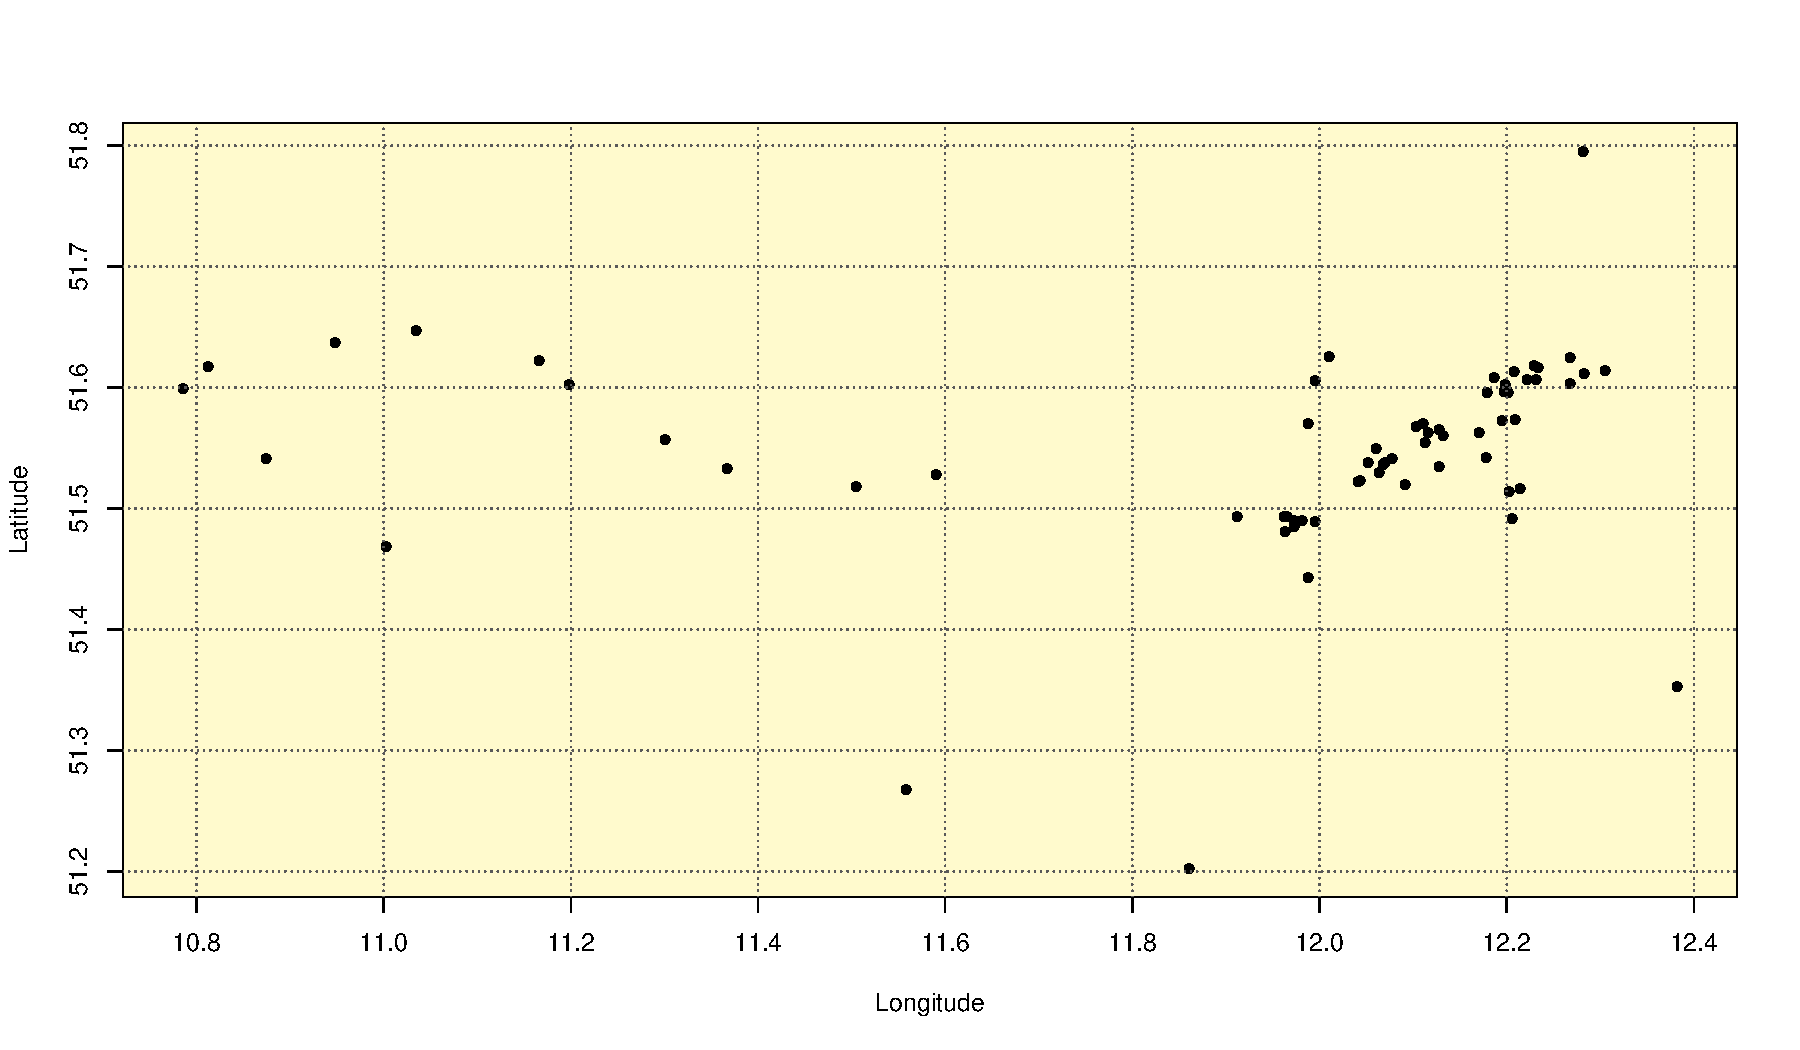
\includegraphics[height=85mm]{cell_locations.pdf}
\end{center}
\end{frame}

\begin{frame}{Mobilfunkzellen}
\begin{center}
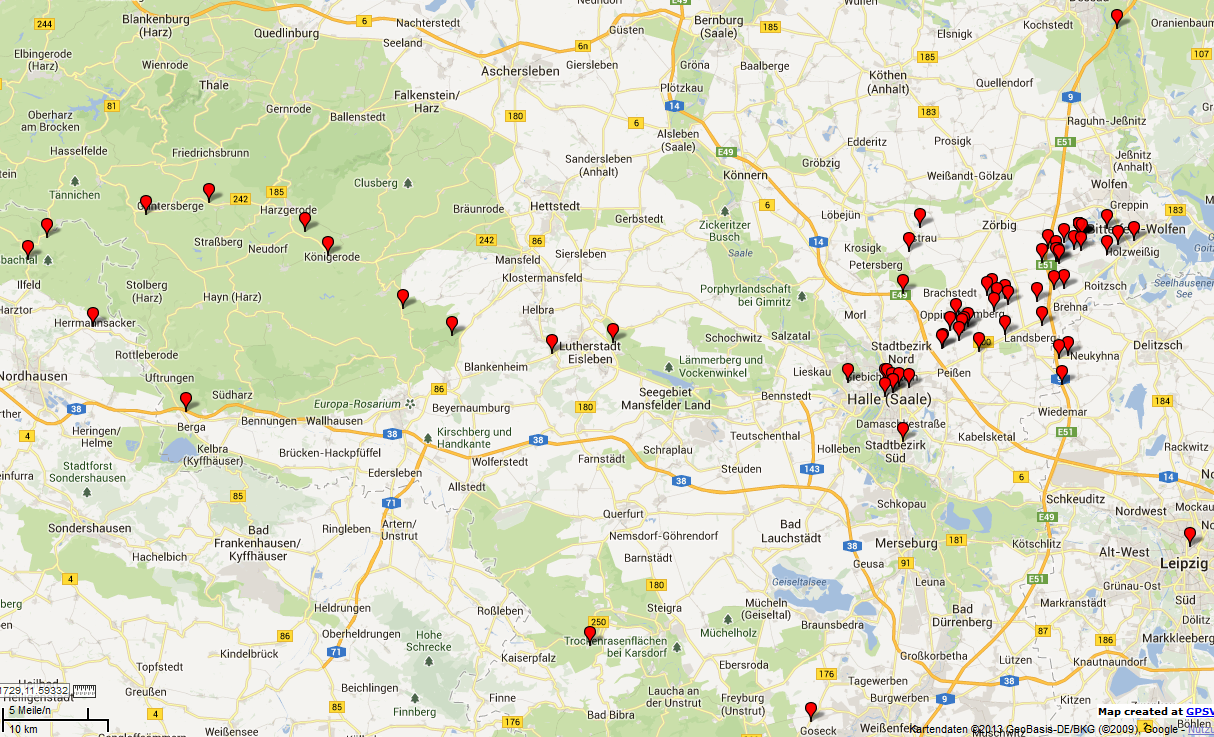
\includegraphics[width=1\linewidth]{map.png}
\end{center}
\end{frame}

\section{Schlussbetrachtung}
\frame{\frametitle{Gliederung} \tableofcontents[currentsection]}
\begin{frame}{Kritische W�rdigung}
\begin{itemize}
\item Daten bisher unverschl�sselt und unkomprimiert gespeichert
\item Ortung nur �ber Mobilfunk
\item nicht alle gesammelten Daten f�r Vorhersage betrachtet
\end{itemize}
\end{frame}

\section{Quellen}
\frame{\frametitle{Gliederung} \tableofcontents[currentsection]}
\begin{frame}[allowframebreaks]
\frametitle{Quellen}
\def\bibfont{\scriptsize}
\printbibliography
\end{frame}

% cite all resources to be printed in bibliography
% this frame will not be shown
\begin{frame}<0>
\frametitle{Quellen}

\end{frame}

\begin{frame}
\thispagestyle{empty}
\begin{center}
\Huge
Vielen Dank f�r Ihre Aufmerksamkeit!\\
Fragen?
\end{center}
\end{frame}

\end{document}



